\documentclass[twocolumn,a4j]{jsarticle}
\bibliographystyle{junsrt}

\setlength{\topmargin}{-20.4cm}
\setlength{\oddsidemargin}{-10.4mm}
\setlength{\evensidemargin}{-10.4mm}
\setlength{\textwidth}{18cm}
\setlength{\textheight}{26cm}

\usepackage[top=15truemm,bottom=20truemm,left=20truemm,right=20truemm]{geometry}
\usepackage[latin1]{inputenc}
\usepackage{amsmath}
\usepackage{amsfonts}
\usepackage{amssymb}
\usepackage[dvipdfmx]{graphicx}
\usepackage[hang,small,bf]{caption}
\usepackage[subrefformat=parens]{subcaption}
\usepackage[dvipdfmx]{color}
\usepackage{listings}
\usepackage{listings,jvlisting}
\usepackage{geometry}
\usepackage{framed}
\usepackage{color}
\usepackage[dvipdfmx]{hyperref}
\usepackage{ascmac}
\usepackage{enumerate}
\usepackage{tabularx}
\usepackage{cancel}
\usepackage{scalefnt}
\usepackage{overcite}
\usepackage{otf}
\usepackage{multicol}
\usepackage[geometry]{ifsym}

\renewcommand{\figurename}{Fig.}
\renewcommand{\tablename}{Table }

\hypersetup{%
    hidelinks %リンクの色消し
}

\lstset{
basicstyle={\ttfamily},
identifierstyle={\small},
commentstyle={\smallitshape},
keywordstyle={\small\bfseries},
ndkeywordstyle={\small},
stringstyle={\small\ttfamily},
frame={tb},
breaklines=true,
columns=[l]{fullflexible},
xrightmargin=0zw,
xleftmargin=3zw,
numberstyle={\scriptsize},
stepnumber=1,
numbersep=1zw,
lineskip=-0.5ex
}

% キャプション後ろのダブルコロンを消す
\makeatletter
\long\def\@makecaption#1#2{%
  \vskip\abovecaptionskip
  \iftdir\sbox\@tempboxa{#1\hskip1zw#2}%
    \else\sbox\@tempboxa{#1 #2}%
  \fi
  \ifdim \wd\@tempboxa >\hsize
    \iftdir #1\hskip1zw#2\relax\par
      \else #1 #2\relax\par\fi
  \else
    \global \@minipagefalse
    \hbox to\hsize{\hfil\box\@tempboxa\hfil}%
  \fi
  \vskip\belowcaptionskip}
\makeatother


\makeatletter
\def\@maketitle
{
\begin{center}
{\LARGE \@title \par}
\end{center}
\begin{flushright}
{\large \@date}\\
{\large M2 \@author}
\end{flushright}
\par\vskip 1.5em
}
\makeatother

\author{来代 勝胤 / KITADAI Masatsugu}
\title{令和5年度 6月度 月例報告書}
\date{2023/06/28}

\begin{document}
\columnseprule=0.1mm
\maketitle

\section*{報告内容}
\begin{enumerate}[1.]
  \item 数値シミュレーションによる計測手法評価
  \item 数値シミュレーション結果
  \item 7月の予定
\end{enumerate}

\section*{進捗報告}
今月は,ISTPの原稿作成に向けた
数値シミュレーション結果の整理および
計測アルゴリズムの検討を行った.

\section{数値シミュレーションによる計測手法評価}
計測アルゴリズムの性能評価として,
数値シミュレーションを用いた誤差評価を行う.
ここでは,3次元の定常解が示された流れ場を用いて
実験条件を再現する.今月は数値シミュレーションの詳細と
その計算結果について報告する.\\

\subsection{再現する回転壁付近の流れ場}
\begin{figure}[htbp]
  \footnotesize
  \begin{center}
    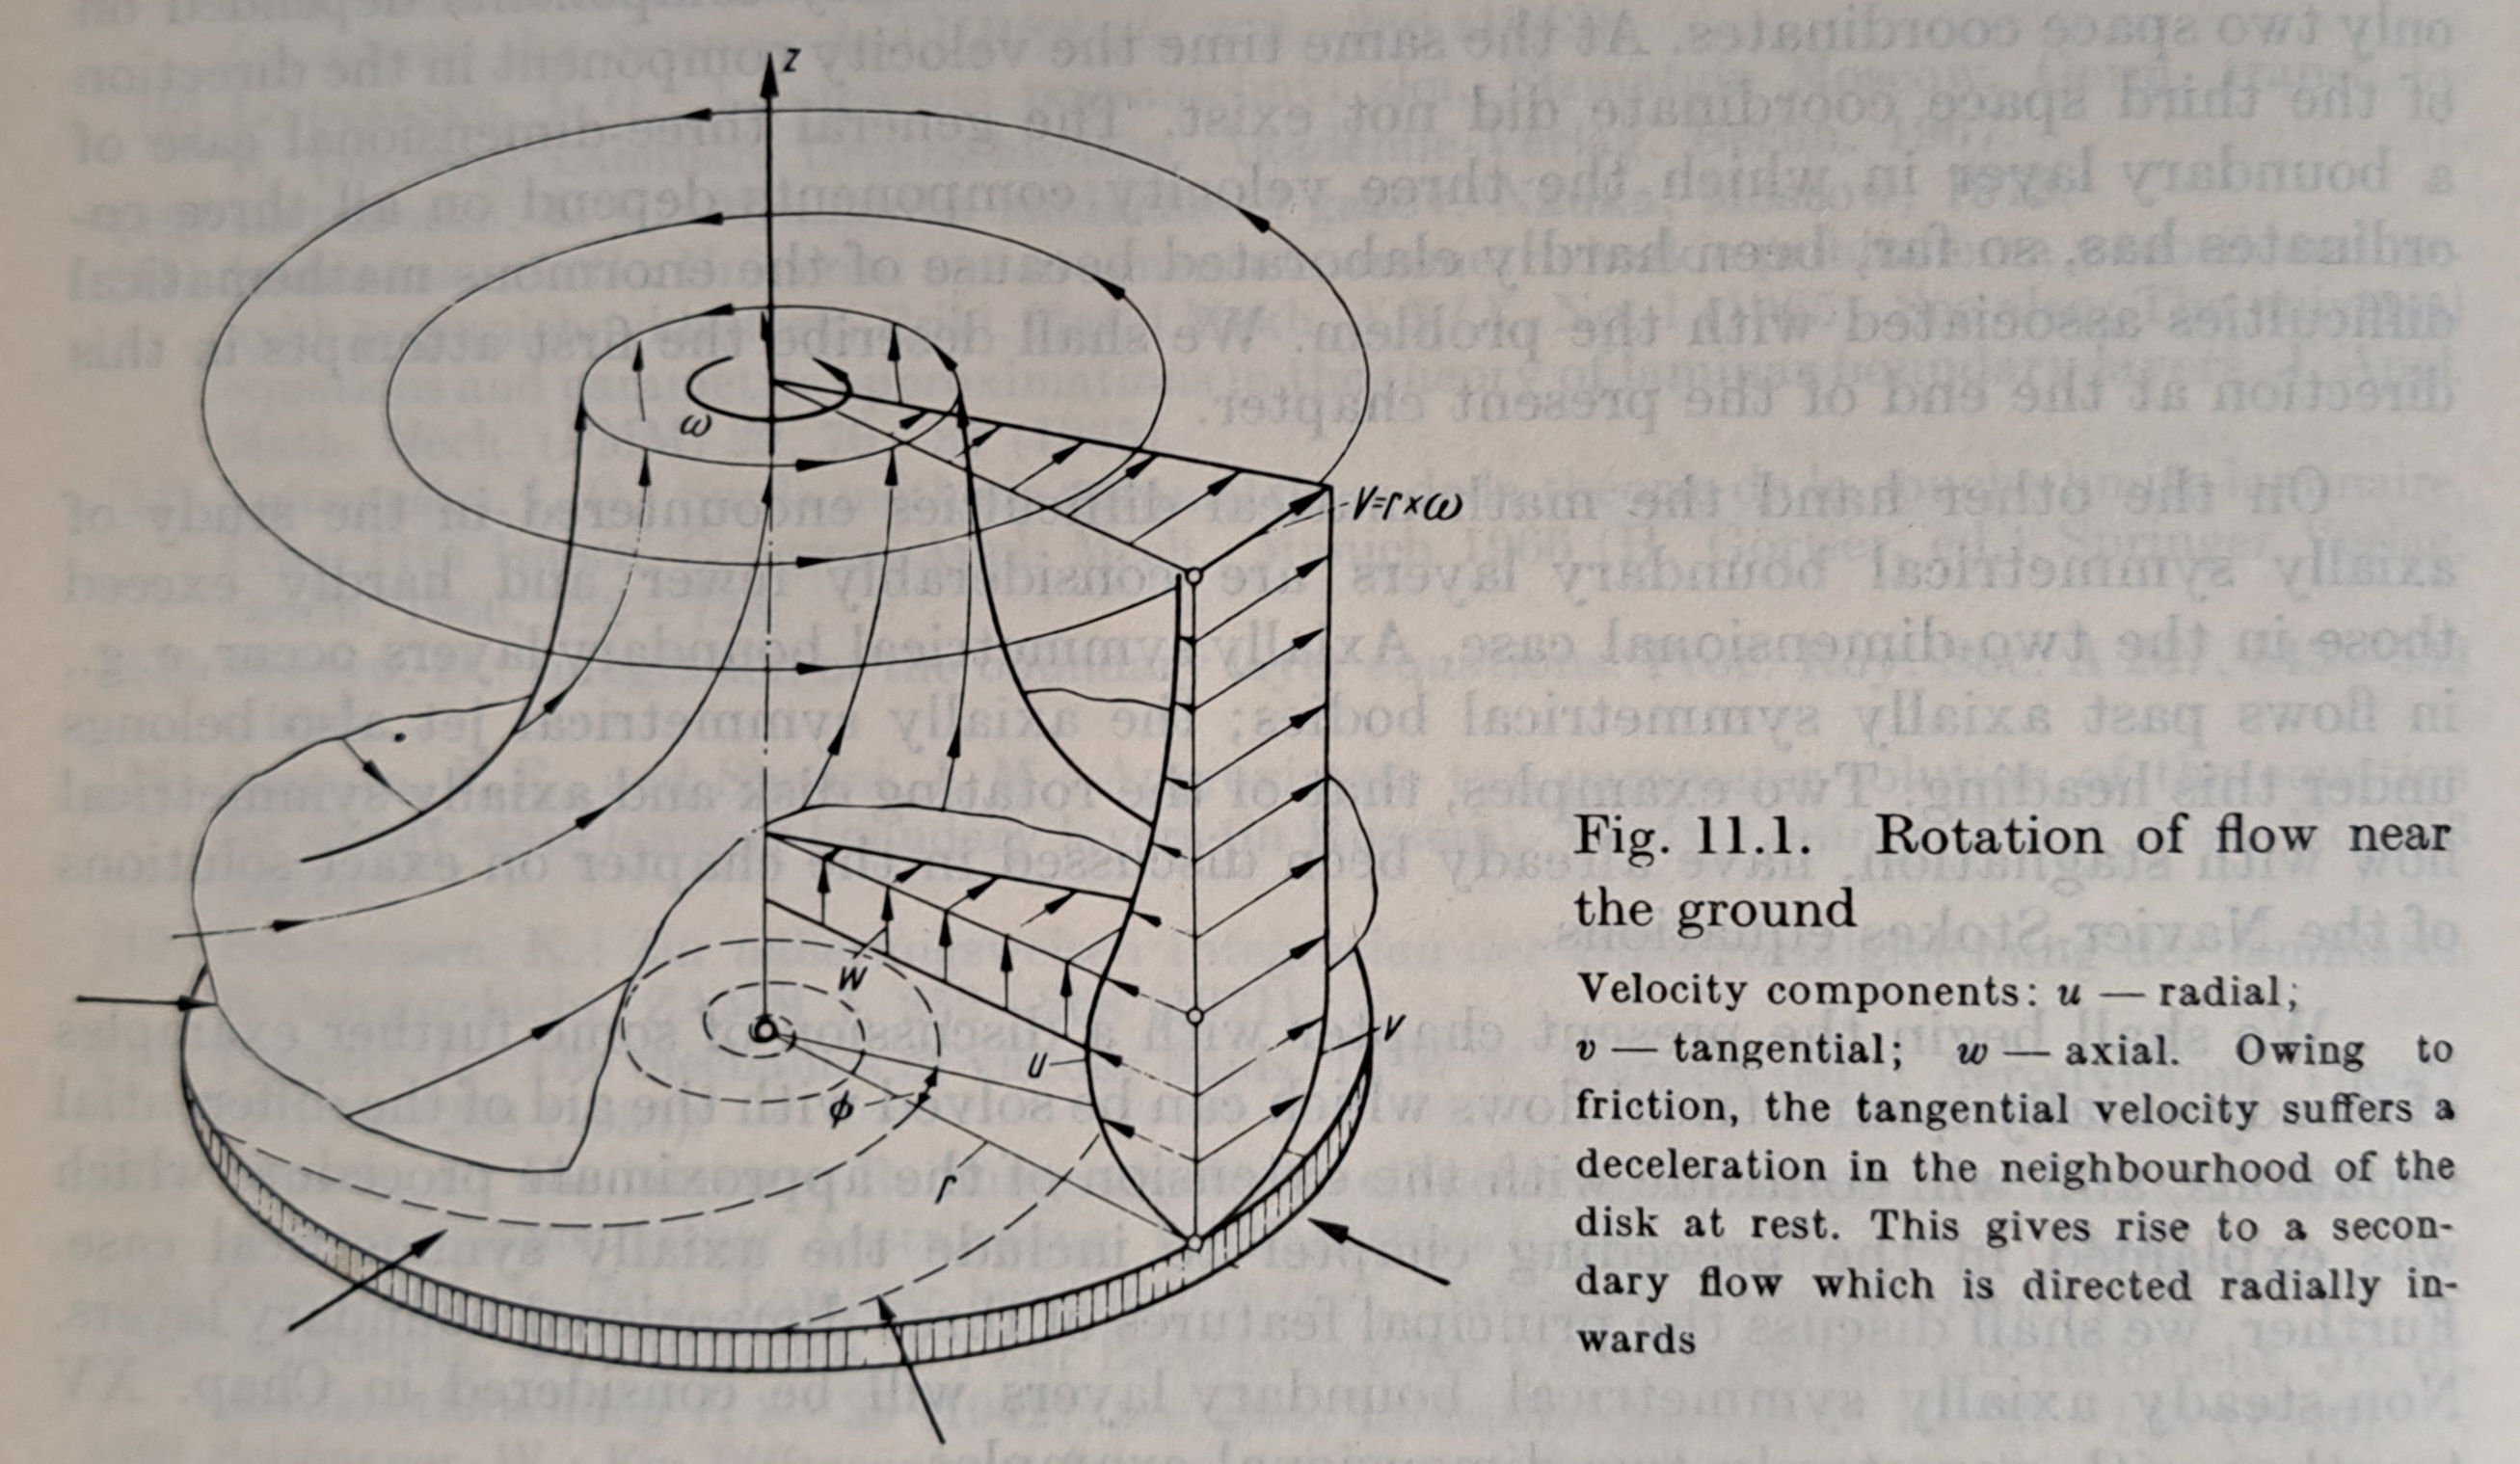
\includegraphics[width=68mm]{../images/Boundary-Layer_Theory_Fig.11.1.jpg}
    \caption{Rotation of flow near the ground}
  \end{center}
\end{figure}

\subsection*{【流れの解析解】}
\begin{eqnarray*}
  \zeta &=& z \sqrt{\frac{\omega}{\nu}}\\
  \\
  V_r &=& r \omega F \left(\zeta\right)\\
  V_\theta &=& r \omega G \left(\zeta\right)\\
  u &=& \sqrt{\nu \omega} H \left(\zeta\right)
\end{eqnarray*}

\subsection*{【境界条件】}
\begin{table}[hbtp]
  \centering
  \begin{tabular}{ c c c c }
    $x=0$      & $V_r=0$ & $V_\theta =0$        & $u=0$ \\
    $x=\infty$ & $V_r=0$ & $V_\theta =r \omega$ &       \\
  \end{tabular}
\end{table}

\newpage

\begin{figure}[htbp]
  \footnotesize
  \begin{center}
    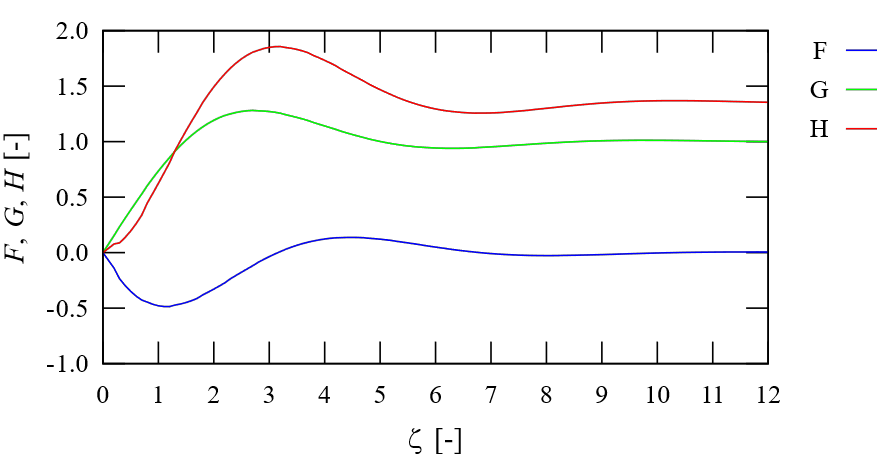
\includegraphics[width=80mm]{../images/FGH.png}
    \caption{$F(\zeta)$, $G(\zeta)$, $H(\zeta)$ の推移}
    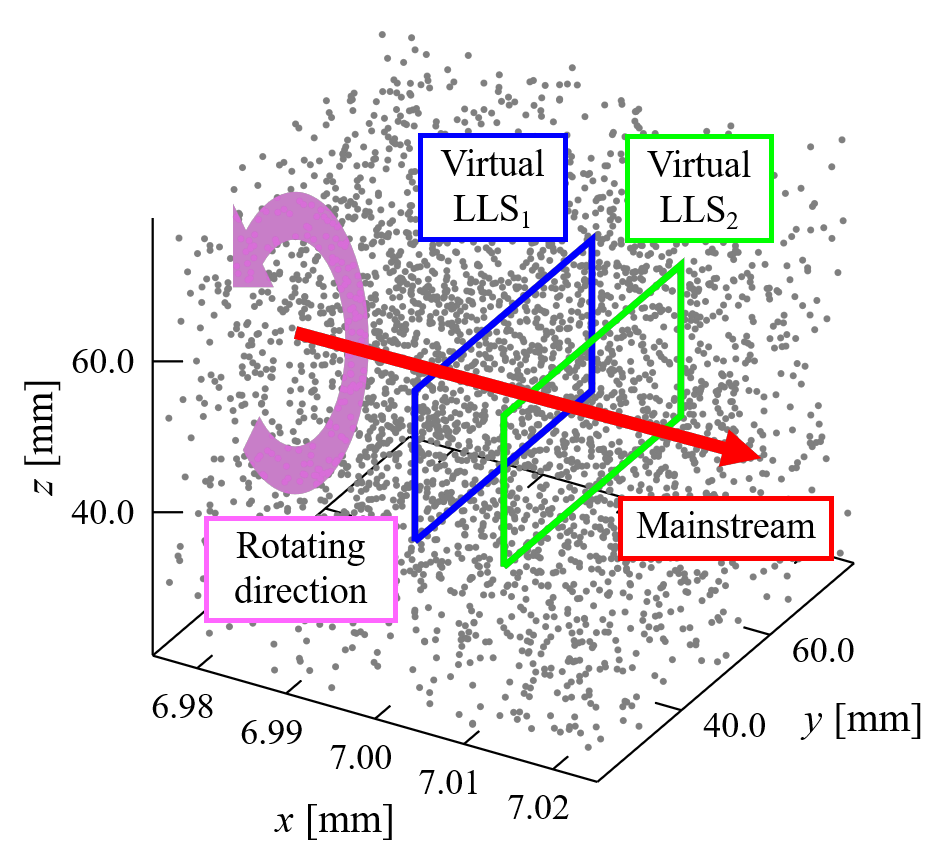
\includegraphics[width=80mm]{../images/Numerical_simulation_of_flow.png}
    \caption{数値シミュレーションの概略図}
  \end{center}
\end{figure}

\section{数値シミュレーションの結果}
\subsection{計測アルゴリズムの適用結果}
数値シミュレーションで用いる流れ場の解析解を
Fig.4に,数値シミュレーションにより作成した粒子像から
計測手法を適用した結果を以下のFig.5に示す.
結果より,解析解と計測結果の反時計回りの二次流れ構造および速度分布は
一致していることがわかる.ここで,Fig.5(a)と(b)を比較すると,
$n_p=500$ のときに誤ベクトルが多く発生していることがわかる.
これは,粒子数の違いにより,
トラッキング時に異なる粒子と対応づいているためと考えられる.

\newpage
\noindent
$\blacksquare$ \textgt{流れ場の解析解}
\begin{figure}[htbp]
  \footnotesize
  \begin{center}
    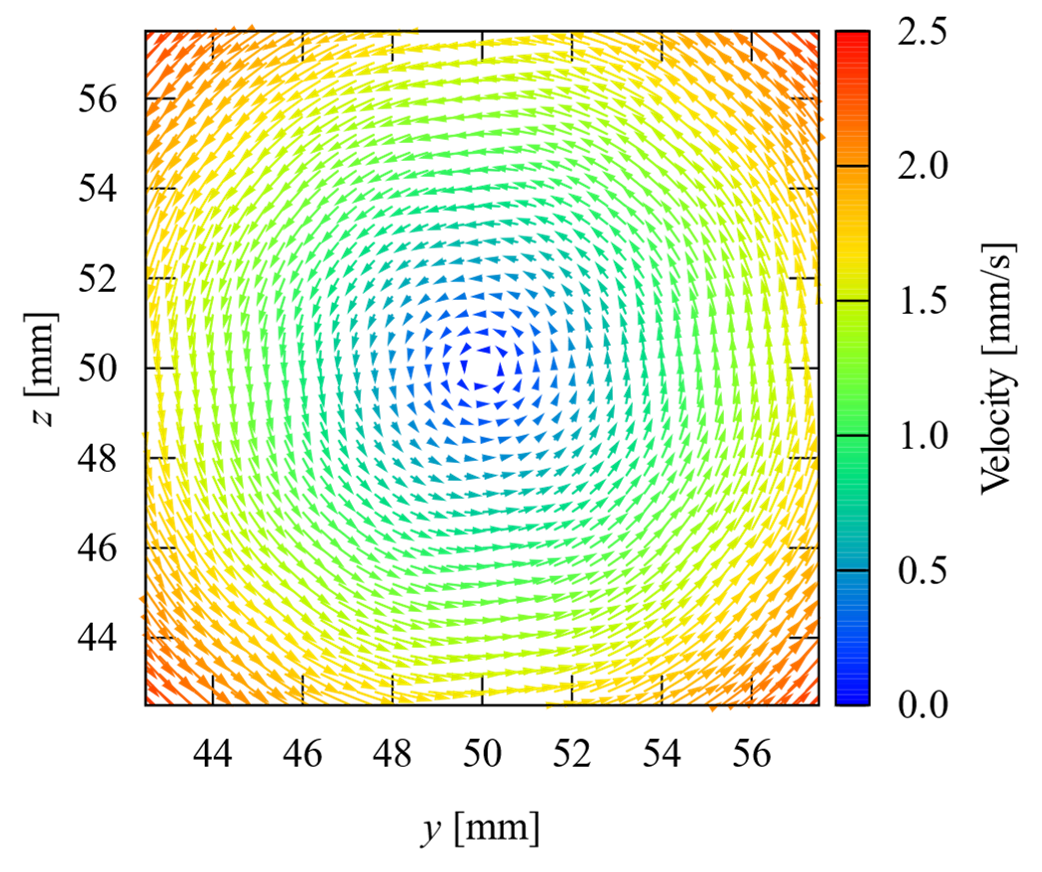
\includegraphics[width=70mm]{../images/velocity_correct.png}
    \caption{Correct velocity}
  \end{center}
\end{figure}

$\blacksquare$ \textgt{PTVの再配置結果}
\begin{figure}[htbp]
  \footnotesize
  \begin{center}
    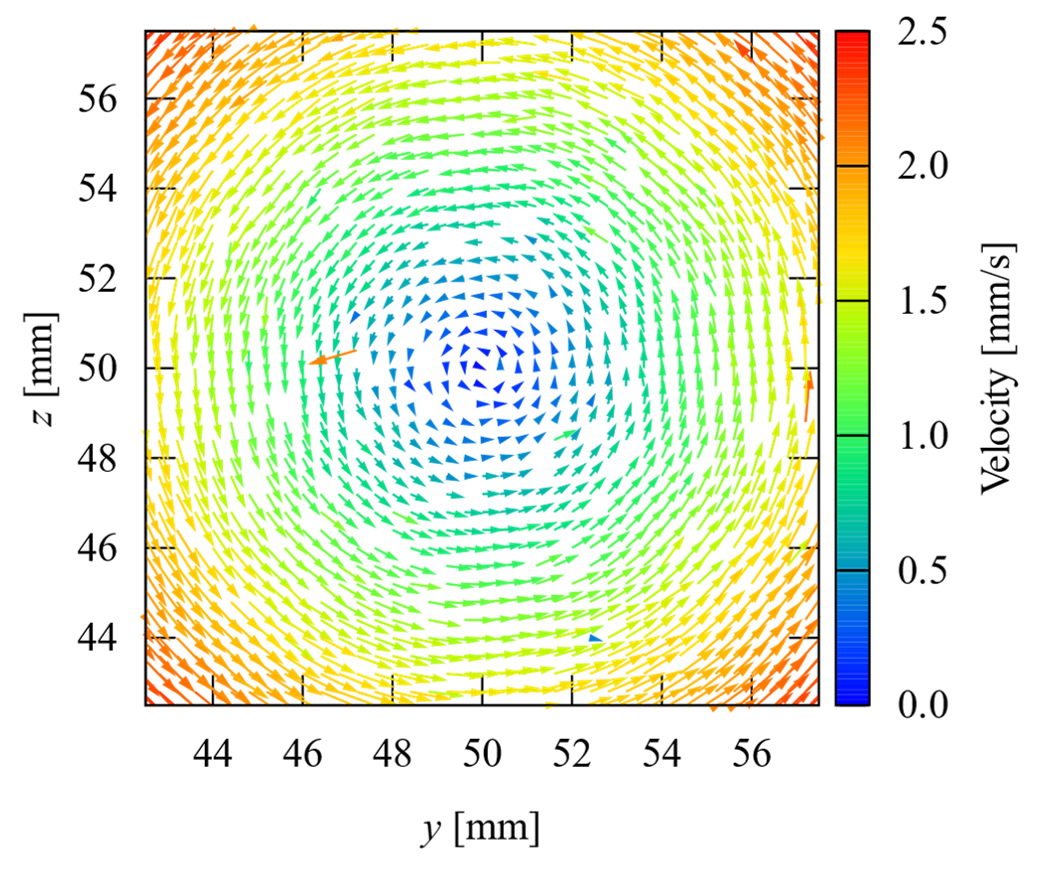
\includegraphics[width=70mm]{../images/velocity_10-50.png}
    \subcaption{$(\omega, n_p) = (10, 50)$}
    \vskip \baselineskip
    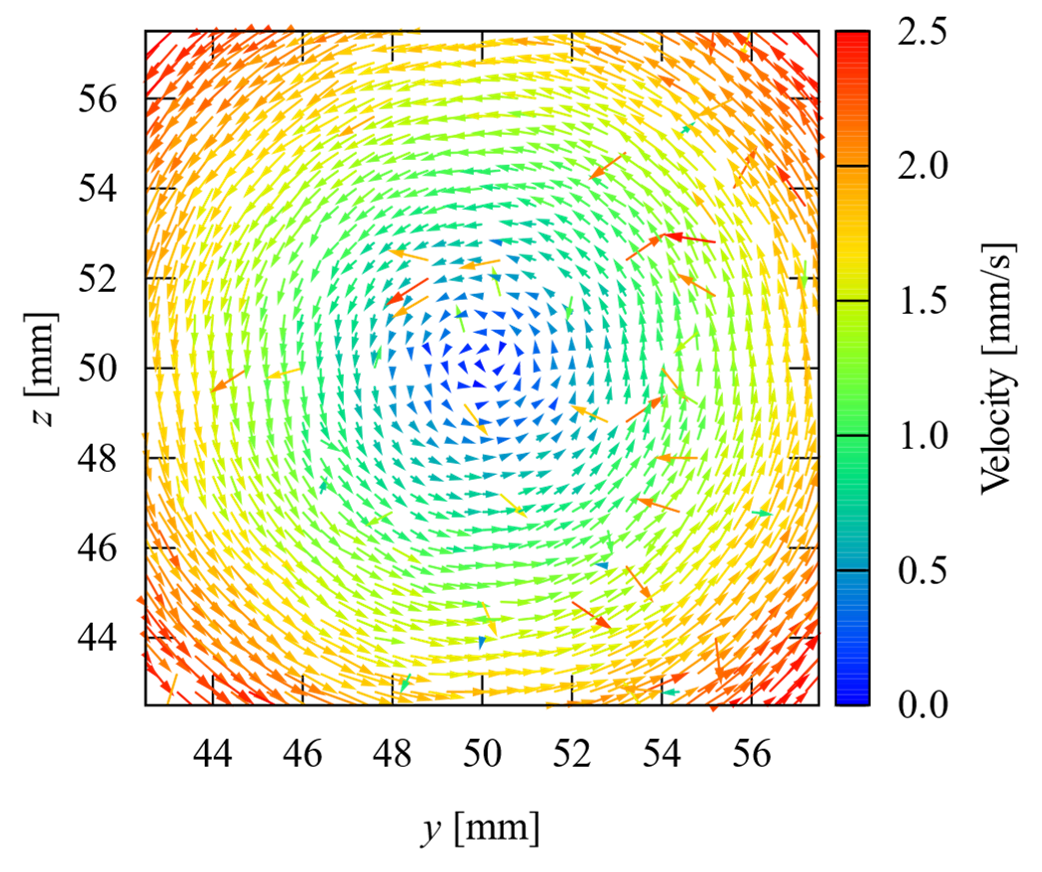
\includegraphics[width=70mm]{../images/velocity_10-500.png}
    \subcaption{$(\omega, n_p) = (10, 500)$}
  \end{center}
  \caption{Time-averaged velocity}
\end{figure}

\newpage
\subsection{RMSE率の計算結果}
ここで,定量的な性能評価を行うため
この計測面内で最大の速度ベクトルとなる
$V_{max}=2.5$ [mm/s]を基準として,
解析解とのRMSE率 $E$ を以下の式から計算する.
また,その結果をFig.6に示す.結果より,
本手法における計測精度は
粒子数の$n_p$が大きく影響することがわかる.
このことから,本手法は誤差率が$5\%$以下を示す
$n_p<= 150$ の範囲で運用することが望ましいと考えられる.\\

\noindent
$\blacksquare$ \textgt{RMSE率の計算}
\begin{eqnarray*}
  E = \frac{RMSE}{V_{max}} \times 100
\end{eqnarray*}

\begin{figure}[htbp]
  \footnotesize
  \begin{center}
    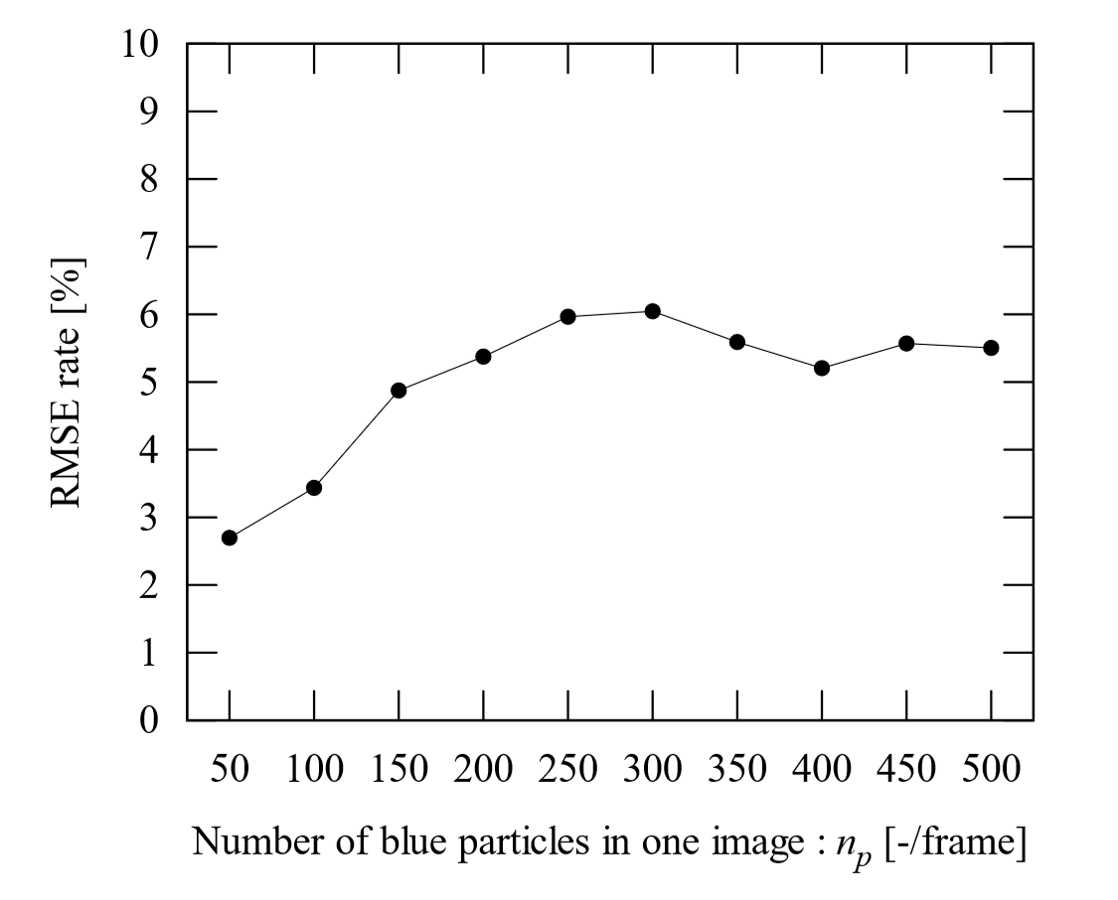
\includegraphics[width=80mm]{../images/error_1.png}
    \subcaption{Difference in $n$}
    \vskip \baselineskip
    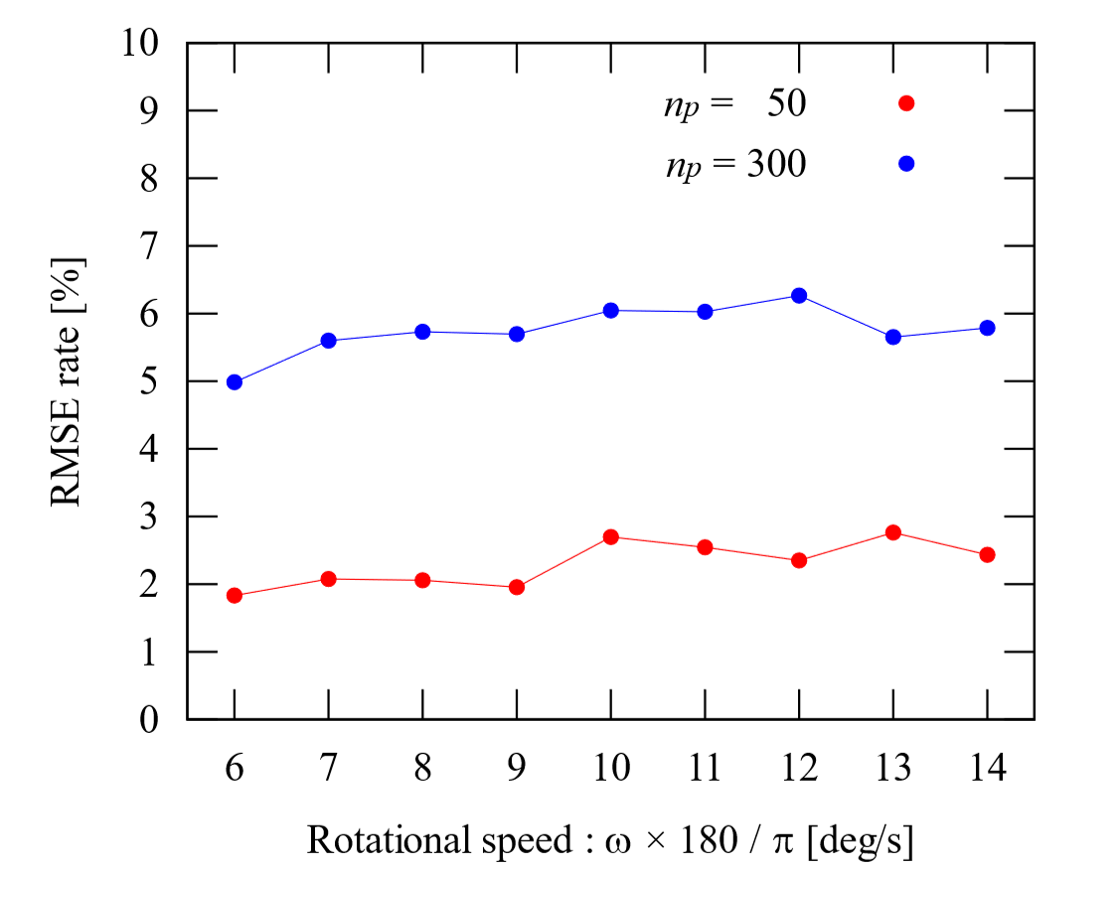
\includegraphics[width=80mm]{../images/error_2.png}
    \subcaption{Difference in $\omega$}
  \end{center}
  \caption{RMSE rate}
\end{figure}

\section{7月の予定}
\begin{itemize}
  \item ISTP 原稿提出 (6/30)
  \item タイヤモデル周りの流れ場測定実験
\end{itemize}

\end{document}